\documentclass[onlymath]{beamer}
%\usepackage[affil-it]{authblk}


\usetheme{default}
\usecolortheme{beaver}

\setbeamercolor{block title}{use=structure,fg=white,bg=structure.fg!75!black}
\setbeamercolor{block body}{parent=normal text,use=block title,bg=block title.bg!10!bg}

\addtobeamertemplate{navigation symbols}{}{%
	\usebeamerfont{footline}%
	\usebeamercolor[fg]{footline}%
	\hspace{1em}%
	\insertframenumber/\inserttotalframenumber
}

%quasi-historischer Header:
\usepackage{verbatim}
\usepackage[utf8]{inputenc}
\usepackage[ngerman]{babel}
\usepackage{ulem}
%\usepackage{scrextend}
%
%\usepackage{microtype} % get rid of bad boxes (overful hbox) in bibliography {https://www.mrunix.de/forums/showthread.php?76019-Biblatex-Overfull-Boxes-im-Literaturverzeichnis-beheben-kein-minimal-bsp}
%
%\usepackage{csquotes} % {"When using babel or polyglossia with biblatex, loading csquotes is recommended to ensure that quoted texts are typeset according to the rules of your main language."} {https://tex.stackexchange.com/questions/229638/package-biblatex-warning-babel-polyglossia-detected-but-csquotes-missing/229653}
%
%\usepackage[backend=biber]{biblatex}
%\addbibresource{bibliography.bib}
%
%%\usepackage{algorithm}
%%\usepackage{algorithmicx}[noend]
\usepackage{bbold}
\usepackage{listings}
\lstset
{ %Formatting for code in appendix
	basicstyle=\footnotesize,
	numbers=left,
	frame=single
	stepnumber=1,
	showstringspaces=false,
	tabsize=1,
	breaklines=true,
	breakatwhitespace=false,
}
%\usepackage[noend]{algpseudocode}
%\usepackage{multicol}
%
%\usepackage[official]{eurosym} % € - Symbol
%
\newcommand{\mc}{Markow-Kette}

\title{Syntaxbasierte Reduktion von PRISM Modellen}
\author{Maximilian Starke}
\institute[VFU] % (optional)
{
	\inst{}%
	Fakultät für Informatik\\
	Technische Universität Dresden
}
\date{\today}


%\logo{\includegraphics[height=1.5cm]{lion-logo.png}}


%
\usepackage{mathtools}
%\usepackage{ragged2e}
%
%\usepackage{framed}
%\usepackage{amsmath, amssymb}
%\usepackage{enumerate}
%\usepackage{tabularx}
%
\DeclareMathOperator*{\argmin}{\arg\min}
%
\usepackage{pgfplots}
\pgfplotsset{width=10cm,compat=1.10}
\usepgfplotslibrary{fillbetween}
%\newcolumntype{P}[1]{>{\centering\arraybackslash}p{#1}}
%
%\usepackage{listings}
%
%\newcolumntype{M}[1]{>{\centering\arraybackslash}m{#1}}
%\newcolumntype{L}[1]{>{\flushleft\arraybackslash}m{#1}}
%
%
\usepackage{tikz}
%\usepackage{verbatim}
%
\usetikzlibrary{%
	arrows,
	shapes,
	shapes.misc,% wg. rounded rectangle
	shapes.arrows,%
	chains,%
	matrix,%
	positioning,% wg. " of "
	backgrounds,
	fit,
	petri,
	scopes,%
	decorations.pathmorphing,% /pgf/decoration/random steps | erste Graphik
	shadows,%
	calc
}
%#1
\tikzstyle{vertex}=[circle, minimum size=20pt, line width = 1pt, draw = black]
\tikzstyle{target} = [vertex, double, double distance = 1pt]
\tikzstyle{edge} = [draw,shorten > = 1pt, shorten < = 1pt, line width=1pt,->]
\tikzstyle{medge} = [draw, line width = 8pt, yellow!50]
\tikzstyle{weight} = [font=\small]
\tikzstyle{selected edge} = [draw,line width=5pt,-,red!50]
\tikzstyle{ignored edge} = [draw,line width=5pt,-,black!20]

\usepackage{relsize}
%
%\usepackage{xcolor}
%% maybe install minted some day and make syntax highlighting###
%
\usepackage[utf8]{inputenc}
\usepackage[ngerman]{babel}
\usepackage{amsmath, amssymb, amsxtra, amsthm}
\usepackage{mathrsfs}
%\usepackage{enumerate}
%\usepackage{multicol} % multiple collums in enumerate
%
%\usepackage[thmmarks,amsmath,hyperref,noconfig]{ntheorem} 
%% erlaubt es, Sätze, Definitionen etc. einfach durchzunummerieren.
\newtheorem{satz}{Satz}[section] % Nummerierung nach Abschnitten
\newtheorem{proposition}[satz]{Proposition}
\newtheorem{korollar}[satz]{Korollar}
%\newtheorem{vermutung}[satz]{Vermutung}
\newtheorem*{partproof}{Beweis.}
%
%\theorembodyfont{\upshape}
%\newtheorem{beispiel}[satz]{Beispiel}
%\newtheorem{bemerkung}[satz]{Bemerkung}
%\newtheorem{algorithmus}[satz]{Algorithmus}
%%%%%%\newtheorem{beweis}[beispiel]{Beweis}

%
%\theoremstyle{nonumberplain}
%\theoremheaderfont{\itshape}
%\theorembodyfont{\normalfont}
%\theoremseparator{.}
%\theoremsymbol{\ensuremath{_\Box}}
%\newtheorem{beweis}{Beweis}
%\newtheorem{beweiss}{Beweisskizze}
%
%\qedsymbol{\ensuremath{_\Box}}
%
%\usepackage{chngcntr}
%\counterwithin{figure}{section}
%
\tikzstyle{block} = [rectangle, draw, fill=blue!40, 
text width=7em, text centered, rounded corners, minimum height=5em, node distance= 4.5cm, line width = 2pt]
%
%
\tikzstyle{cblock} = [rectangle, draw, fill=blue!40, 
text width=7em, text centered, rounded corners, minimum height=5em, node distance= 3.0cm, line width = 2pt]
%
%
\tikzstyle{line} = [draw, -latex', line width = 1pt]
%
%
\tikzstyle{cloud} = [ fill = white, rectangle, draw, rounded corners, node distance=2cm,
minimum height=2.5em]
%
\pgfdeclarelayer{bg}
\pgfsetlayers{bg,main}	
%
\pgfdeclarelayer{foreground}
\pgfdeclarelayer{background}
%% tell TikZ how to stack them (back to front)
\pgfsetlayers{bg,background,main,foreground}
%
%\newenvironment{meta}
%{\begin{center} \Large \color{red} META: \hspace{2ex} \large \color{blue}}
%	{\end{center}}
%

\AtBeginSection{\frame{\sectionpage}}
\AtBeginSubsection{\frame{\subsectionpage}}
\begin{document}	

\frame{\titlepage}

%\begin{frame}
%	\frametitle{Inhalt}
%	\tableofcontents
%\end{frame}


\section{Einführung}



\begin{frame}
	\frametitle{Motivation}
	\begin{itemize}
		\item probabilistische Modelle: z.B. \mc{}n
		\item Analyse von Modellen: PRISM model checker \pause
		\item \textbf{$\Rightarrow$ Modellreduktion} \pause $\dots$ basierend auf $\dots$ \begin{itemize}
			\item Bisimulation
			\item Symmetrie \pause
			\item Syntax: Live Range Analysis
		\end{itemize}
	\end{itemize}
\end{frame}



\begin{frame}
	\frametitle{Modellreduktion durch Live Range Analysis}
	\begin{itemize}
		\item Reduktion der Anzahl von Variablen \pause
		\item Invarianz der Reduktion bezüglich gewissen Modelleigenschaften \pause
		\item Ausblick: \begin{itemize}
			\item Grundlagen der Reduktion \pause
			\item Anwendung der Live Range Analysis \pause
			\item Graphfärbung durch Heuristiken \pause
			\item Implementierung in C++ 
			\item Vergleich der reduzierten Modelle
			
		\end{itemize}
	\end{itemize}
\end{frame}

\section{unser Modell}

\begin{frame}[fragile]
	\frametitle{PRISMs Eingabesprache}
%	\scalebox{0.5}{
%\makebox[0pt]{
%	\footnotesize
  \lstset{basicstyle=\footnotesize}
	\begin{lstlisting}
	dtmc
	
	global cf : [0 .. 5]; global a : [0 .. 4];
	global b : [0 .. 4]; global c : [0 .. 4];
	global d : [0 .. 4]; global e : [0 .. 4];
	
	init
	(cf=0) & (a=0) & (b=1) & (c=2) &
	(d=0 | d=1) & (e=4 | e=2)
	endinit
	
	module some_module
	[goto_1] cf = 0 & a = 0 ->   0.4 : cf' = 1 & a' = 1
	+ 0.6 : cf' = 2 & b' = 3;
	[goto_2] cf = 0 & a = 4 ->   0.2 : cf' = 2 & b' = 4
	+ 0.8 : cf' = 4 & e' = 0;
	...
	endmodule
	
	formula failure = (e = 0);
	\end{lstlisting}
%}
%}
\end{frame}


\begin{frame}
	\frametitle{unsere Annahmen}	
\begin{enumerate}[(a)]
	\item Es gibt eine Variable, die als Kontrollflussvariable dient, wir nennen diese hier $cf$ (engl. für \textit{control flow}). \pause
	\item In jeder Transition ist $cf$ in der Eintrittsbedingung eindeutig festgelegt. In allen Folgezustandsbedingungen steht $cf$ eindeutig fest: Dazu bekommt $cf$ entweder explizit einen eindeutigen Wert zugewiesen oder bleibt unverändert. \pause
	\item Es gibt eine Liste von Variablen, die von der Reduktion auszuschließen sind.
\end{enumerate}

\end{frame}


\begin{frame}
	\frametitle{unsere Annahmen}	
	\begin{enumerate}[(d)]
		\item Variablen mit jeweils endlichem Wertebereich $cf \in D_{cf}, x_1 \in D_{1}, x_2, \in D_2, \dots, x_n \in D_n$. \pause
		\item endlich viele Transitionen $t_1, t_2, \dots , t_m$ als Paare von Eintrittsbedingung und Tupel der Folgezustandsbedingungen:
		\[t_i = (f^{enter}_i, (f^{leave}_{i,1}, f^{leave}_{i,2}, \dots , f^{leave}_{i,k_i}))\] \pause
		\item eine Startzustandsbedingung siehe Zeile 7-10.
	\end{enumerate}	
\end{frame}

\begin{frame}
	\frametitle{Optimierung}
	aus ...
	\begin{equation*}
	t_i = (f^{enter}_i, (f^{leave}_{i,1}, f^{leave}_{i,2}, \dots , f^{leave}_{i,k_i}))
	\end{equation*}
	\pause
	wird ...
	\begin{align*}
	t_i^1 & = (f^{enter}_i, (f^{leave}_{i,1})) \\ 
	\onslide<3->{t_i^2 & = (f^{enter}_i, (f^{leave}_{i,2}))\\ }
	\onslide<4->{& \dots \\
	t_i^{k_i} &= (f^{enter}_i, (f^{leave}_{i,k_i})) }
	\end{align*}
\end{frame}

\begin{frame}
	\frametitle{Multigraph}
	\centering
	 $G = (V,E,\cdot_{\mathrm{from}}, \cdot_{\mathrm{to}})$ \pause
\begin{definition}[Multigraph]
	Sei $V \neq \emptyset$ eine nichtleere Menge, aufgefasst als Menge von Knoten \pause und $E$ eine Menge, aufgefasst als Menge gerichteter Kanten. \pause
	Seien weiterhin
	\begin{align*}
	\cdot_{\mathrm{from}} &: E \to V : e \mapsto e_{\mathrm{from}}\text{,} \\
	\cdot_{\mathrm{to}} &: E \to V : e \mapsto e_{\mathrm{to}}
	\end{align*} \pause
	zwei Abbildungen, die jeder Kante $e$ ihren Startknoten $e_{\mathrm{from}}$ sowie ihren Endknoten $e_{\mathrm{to}}$ zuordnen. \pause
	Dann nennen wir $G = (V,E,\cdot_{\mathrm{from}}, \cdot_{\mathrm{to}})$ einen (gerichteten) Multigraph.
\end{definition}
\end{frame}

\begin{frame}
	\frametitle{unser Multigraph}
	\centering
	\framebox[20ex]{	$G = (V,E,\cdot_{\mathrm{from}}, \cdot_{\mathrm{to}})$ } \pause
	\vspace{3ex}
	\begin{enumerate}[(a)]
		\item Transitionen $e^j = (f_j^{enter}, f_j^{leave}) \in E$ \pause
		\item $V\coloneqq D_{cf}$ \pause
		\item $\forall e^j \in E : e^j_{\mathrm{from}} \coloneqq v_1\text{, falls } f_j^{enter} \implies cf = v_1$ \pause
		\item $\forall e^j \in E : e^j_{\mathrm{to}} \coloneqq v_2\text{, falls } f_j^{leave} \implies cf = v_2$
	\end{enumerate}
\end{frame}

\section{Live Range Analysis}

\begin{frame}
	\frametitle{Liveness}
	\begin{itemize}
		\item Compilerbau \pause $\rightarrow$ Registerallokation \pause
		\item Zuordnung von Variablen zu Registern \pause
		\item Wert der Variable $x$ wird noch gebraucht $\Leftrightarrow$ $x$ ist live \pause
	\end{itemize}
	\begin{definition}[Liveness]
		Eine Variable \textit{x} heißt \textit{live} in einem Knoten \textit{v}, wenn es einen in $v$ beginnenden Pfad in $G$ gibt, auf welchem $x$ gelesen wird, ohne dass zuvor auf diesem Pfad $x$ geschrieben wird. Wir schreiben dann $\textrm{live}_x(v)$ und sonst $\neg \textrm{live}_x(v)$.
	\end{definition}
\end{frame}

\newcommand{\mgtup}{$G = (V,E,\cdot_{\mathrm{from}}, \cdot_{\mathrm{to}})$}
\newcommand{\subfrom}{_{\mathrm{from}}}
\newcommand{\subto}{_{\mathrm{to}}}

\begin{frame}
	\frametitle{Pfade in Multigraphen}
	\begin{definition}[Pfad]
		Sei \mgtup{} ein Multigraph. Wir nennen ein Tupel $(v_0,v_1, \dots, v_n)$ von Knoten einen \emph{Pfad} in $G$, wenn für jede zwei aufeinander folgenden Knoten eine solche Kante existiert:
		\begin{equation*}
		\forall i \in \{0, \dots, n-1\} \exists e \in E : v_i = e\subfrom \land v_{i+1} = e\subto
		\end{equation*}
		Wir sagen, dass ein solcher Pfad in einem Knoten $v$ \emph{beginnt}, wenn $v_0 = v$.
	\end{definition}
\pause
\begin{itemize}
	\item CPU Register \pause $\leftrightarrow$ zusammengefasste Variable
\end{itemize}
\end{frame}

\begin{frame}
	\frametitle{Live Range}
	\begin{definition}[Live Range]
		Zu einem Programmgraph \mgtup{} bezeichnen wir mit $\textrm{live\_range}(x)$ für eine Variable $x$ die Menge aller Knoten $v\in V$, sodass $x$ live ist in $v$:
		\[
		\textrm{live\_range}(x) \coloneqq \{v\in V \mid \textrm{live}_x(v) \}
		\]
	\end{definition}
\begin{itemize}
	\item disjunkte Live Ranges \pause $\leftrightarrow$ gleiches Register \pause $\leftrightarrow$ gemeinsame Variable \pause
	\item iterative Berechnung von $\textrm{LIVE}_v \coloneqq \{ x \in \mathrm{Var} \mid \textrm{live}_x(v) \}$ ...
\end{itemize}
\end{frame}

\begin{frame}
	\frametitle{Live Range Analysis}
	Sei $e$ eine Kante (Transition). \pause
	\begin{align}
	\mathrm{GEN}_{e} & \coloneqq \{x \in \mathrm{Var} \mid \text{$x$ gelesen, nicht zuvor $x$ geschrieben in $e$} \} \nonumber \\ 
	\mathrm{KILL}_{e} & \coloneqq \{x \in \mathrm{Var} \mid \text{$x$ geschrieben, nicht zuvor $x$ gelesen in $e$} \} \nonumber
	\end{align}
	\onslide<5->{
	\begin{equation*}
	\mathrm{LIVE}^{in}_{e} = \mathrm{GEN}_{e} \cup \big( \mathrm{LIVE}^{out}_{e} \setminus \mathrm{KILL}_{e} \big) 
	\end{equation*}
	}

	\begin{itemize}
		\onslide<3->{\item $\mathrm{GEN}_{e}$ ... Variablen, die vor $e$ live werden (bleiben).}
		\onslide<4->{\item $\mathrm{KILL}_{e}$ ... Variablen, die vor $e$ dead werden (bleiben).}
		\onslide<6->{\item $\mathrm{LIVE}^{in}_{e}$ ... Menge der live Variablen unmittelbar vor $e$}
		\onslide<7->{\item $\mathrm{LIVE}^{out}_{e}$ ... Menge der live Variablen unmittelbar nach $e$}
	\end{itemize}
	\onslide<8->{
	\begin{equation*}
	\mathrm{LIVE}^{out}_{e} = \bigcup_{f \in E \textrm{ mit } f\subfrom = e\subto} {\mathrm{LIVE}^{in}_{f}  }
	\end{equation*}
	}
\end{frame}

\begin{frame}
	\frametitle{Live Range Analysis (2)}
	\onslide<1->{
		\begin{equation*}
		\textrm{LIVE}_v = \bigcup_{f \in E \textrm{ mit } f\subfrom = v} {\mathrm{LIVE}^{in}_{f}  }
		\end{equation*}
	}
	
	\begin{itemize}
		\onslide<2->{\item Starte mit $\mathrm{LIVE}^{out}_{e} \coloneqq \emptyset$ und $\mathrm{LIVE}^{in}_{e} \coloneqq \emptyset$ für alle Kanten $e \in E$ }
		\onslide<3->{\item Aktualisiere schrittweise anhand der Gleichungen}
		\onslide<4->{\item $x \in \textrm{LIVE}_v \Leftrightarrow \textrm{live}_x(v) \Leftrightarrow v \in \textrm{live\_range}(x)$ }
		\onslide<5->{\item Variablen zusammenfassen, falls $\textrm{live\_range}(x) \cap \textrm{live\_range}(y) = \emptyset$}
	\end{itemize}

\end{frame}

\begin{frame}
	\frametitle{Reduktion des Modells}
	\begin{itemize}
		\onslide<1->{\item $x_1, \dots , x_n$ zusammenfassen zu $y \in (D_{x_1} \cup \dots \cup D_{x_n})$ }
		\onslide<2->{\item alle Vorkommen von $x_1, \dots$ ersetzen}
		\onslide<3->{\item Logik-Widersprüche in Bedingungen auflösen: \pause $x_1 = 1 \land x_2 = 5$ }
	\end{itemize}
\onslide<4->{ Aber welche Variablen sollen wir zusammenfassen?}
\begin{itemize}
\onslide<5->{	\item maximale Reduktion $\leftrightarrow$ minimale Zahl an Variablen}
\onslide<6->{	\item $\rightarrow$ optimale Graphfärbungen finden}
\end{itemize}
	
\end{frame}

\begin{frame}
	\frametitle{Maximale Reduktion $\leftrightarrow$ minimale Zahl an Variablen $\leftrightarrow$ optimale Färbung der Graphen $H$}
	\begin{itemize}
		\onslide<1->{\item Sei $H=(\mathrm{Var}, F)$ ein ungerichteter Graph:}
		\begin{itemize}
			\onslide<2->{\item $\mathrm{Var}$ ... Menge der Variablen des Modells}
			\onslide<3->{\item $\{x,y\} \in F :\Leftrightarrow x \neq y \land \exists v \in D_{cf} : \{x, y\} \subseteq \textrm{LIVE}_v$}
			\onslide<4->{\item d.h. Kanten zwischen Variablen, die irgendwo gleichzeitig live sind }
		\end{itemize}
		\onslide<5->{\item Zusammenfassen von Variablen mit gleicher Farbe }
	\end{itemize}	
\end{frame}

\begin{frame}
	\frametitle{C++ Implementierung}
	\begin{itemize}
		\item Modell parsen \pause
		\item Mengen von zusammenführbaren Variablen berechnen \pause
		\item Mengen mit Farben identifizieren. \pause
		\item Färbung als Reduktion auf das originale Modell anwenden \pause
		\item Heuristiken zum Färben von Graph $H$ anwenden \pause
		\item \textbf{INSBESONDERE: alle reduzierten Modelle mit minimaler Zahl an Variablen auflisten}
	\end{itemize} \pause
	{\LARGE Details der Implementierung später...}
\end{frame}

\section{Ergebnisse der Experimente}

\begin{frame}
	\frametitle{Heuristiken zur Graphfärbung (1): Welsh-Powell Algorithmus}
	\centering
	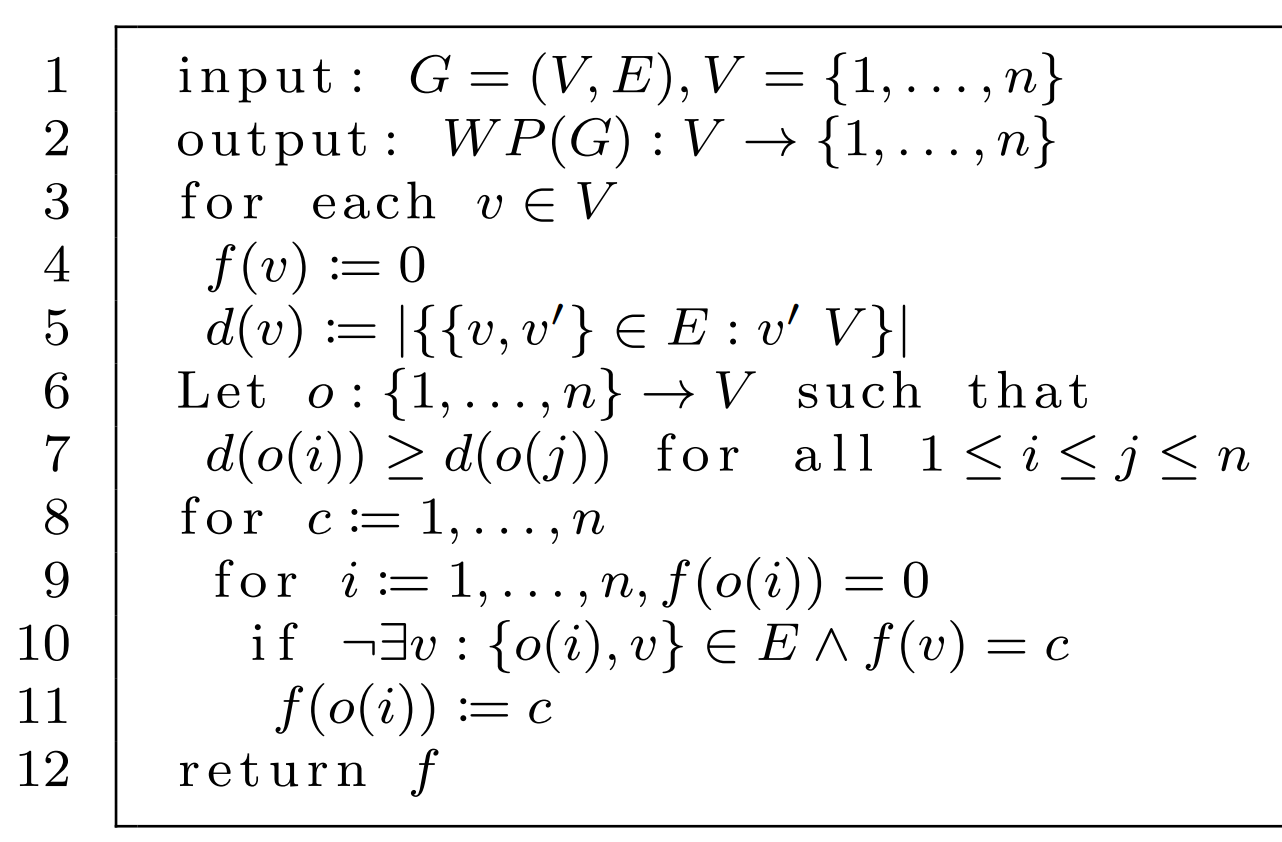
\includegraphics[scale=0.3]{wp.png}
\end{frame}

\begin{frame}
	\frametitle{Heuristiken zur Graphfärbung (2): Remove Nodes Algorithmus}
	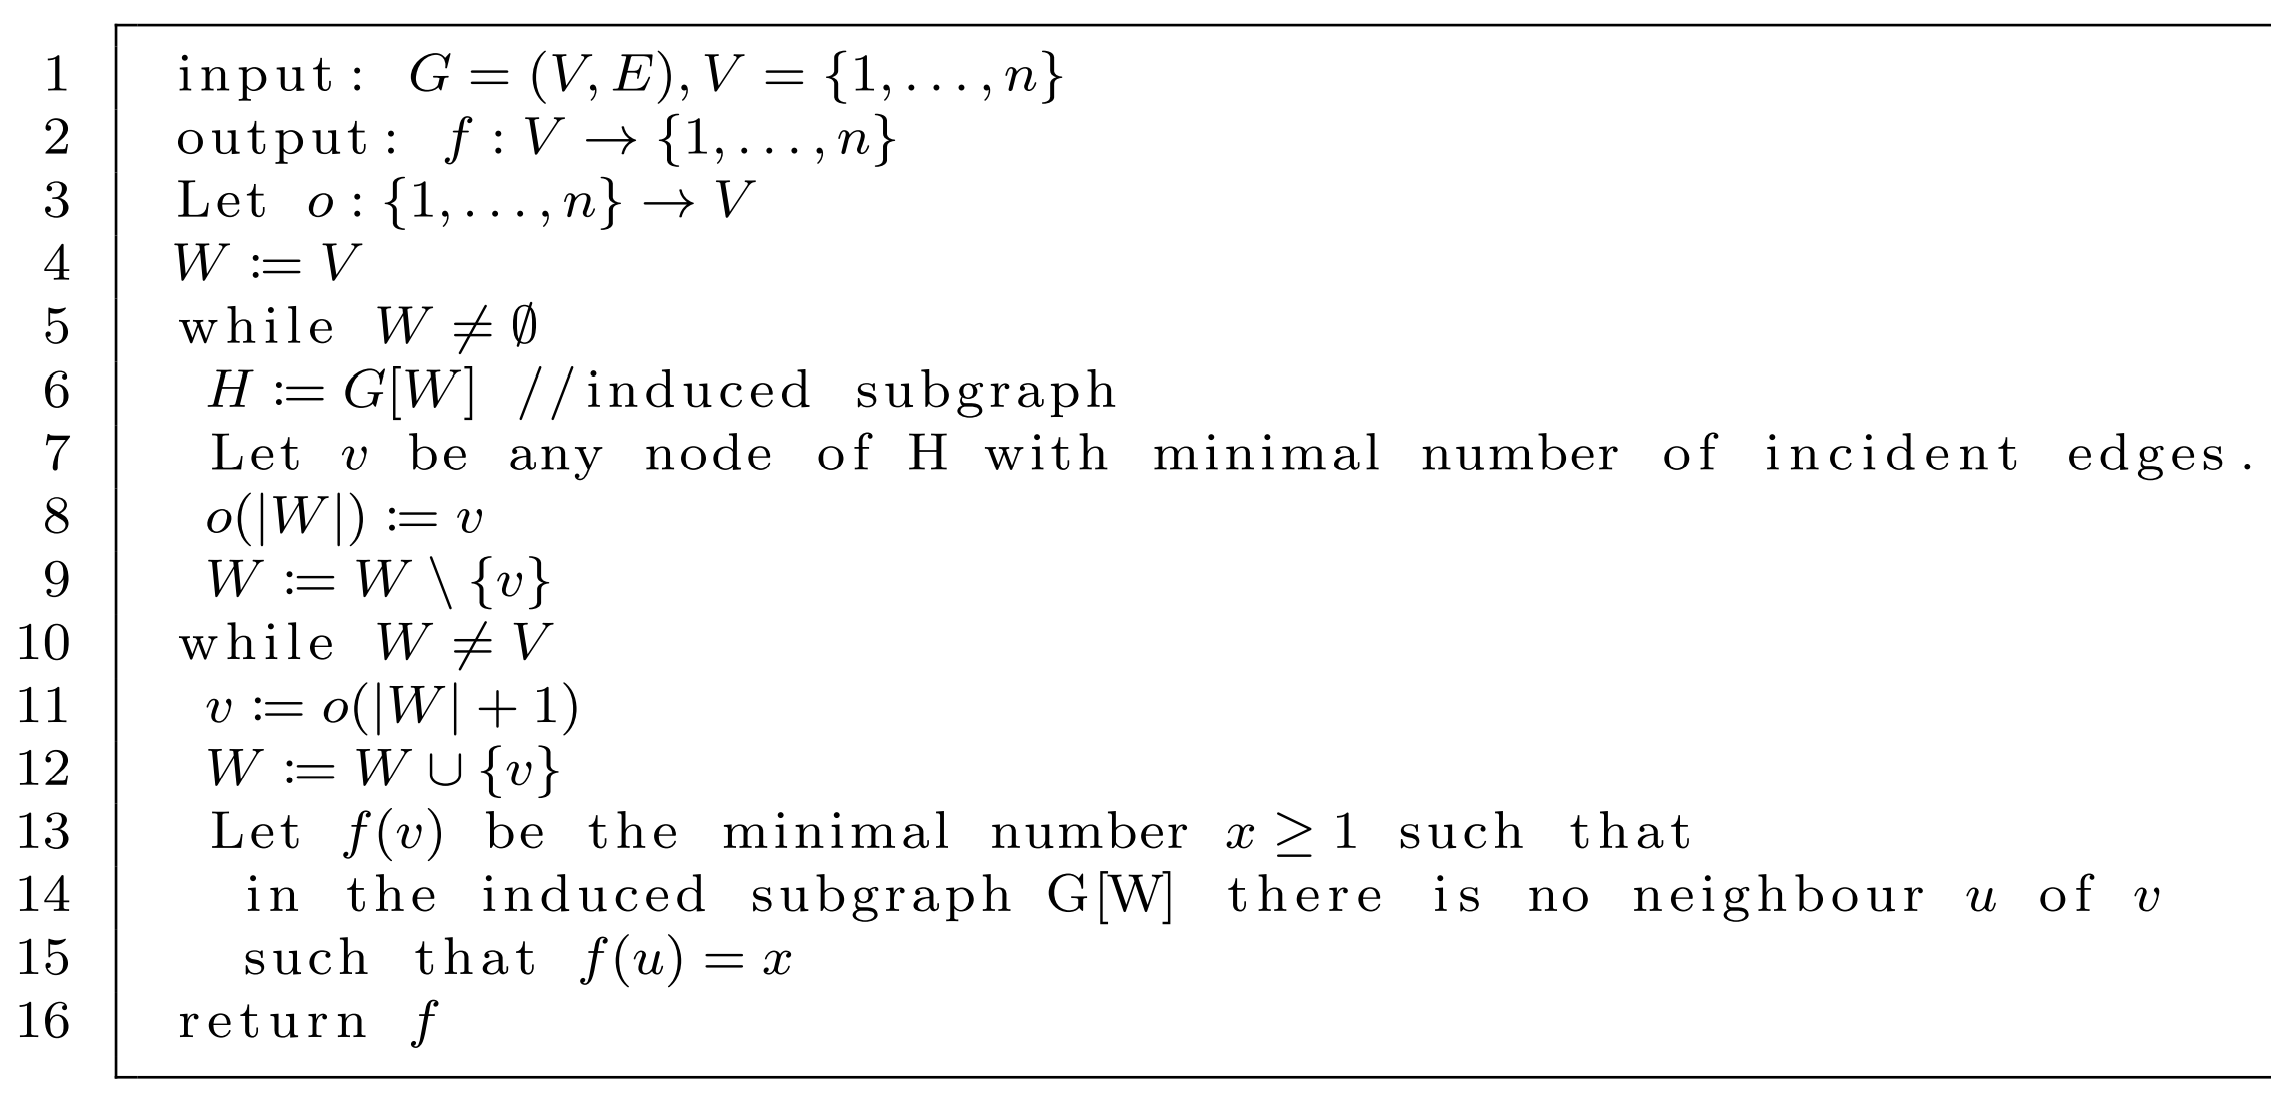
\includegraphics[scale=0.18]{rn.png}
	\begin{itemize}
	\item basierend auf der Idee von Chaitin's Algorithmus zur Graphfärbung
	\item entferne den Knoten mit minimaler Zahl inzidenter Kanten
\end{itemize}
\end{frame}

\begin{frame}
	\frametitle{Heuristiken zur Graphfärbung (3): Maximum Merge First}
	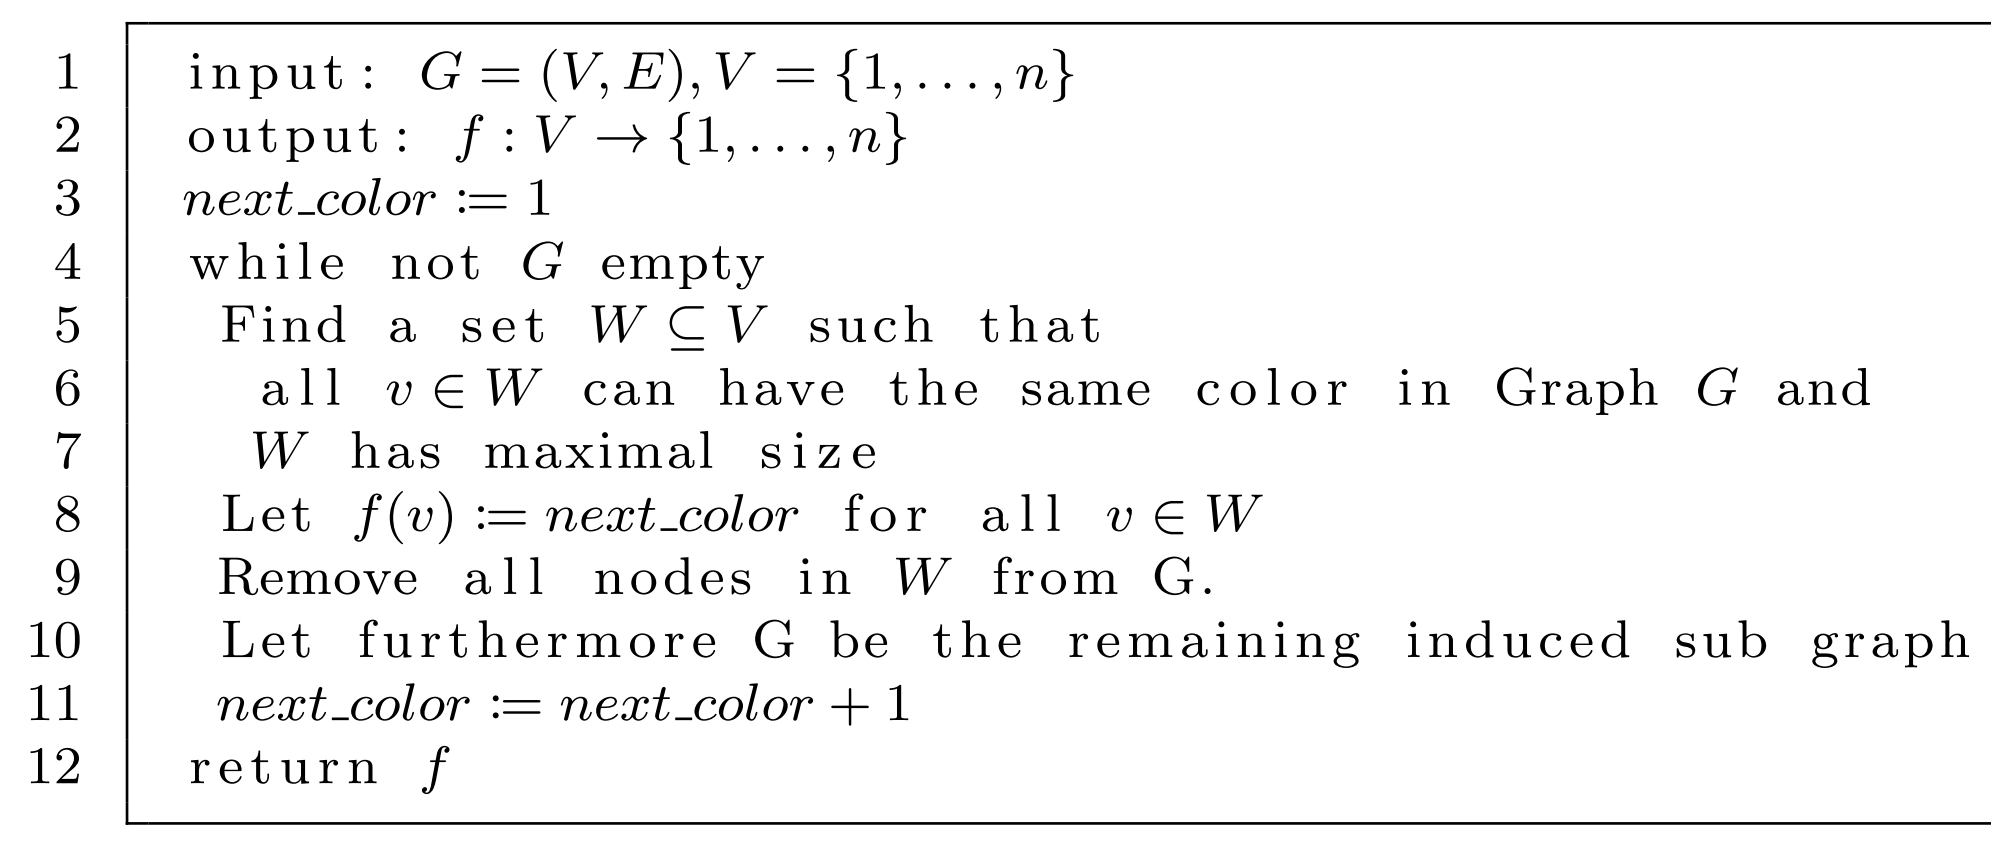
\includegraphics[scale=0.2]{mmf.png}
	\begin{itemize}
		\item (ohne Angabe wie dies im Detail umzusetzen geht)
	\end{itemize}
\end{frame}

\begin{frame}
	\frametitle{Ergebnisse Modell 6}
	\centering
				\makebox[0pt]{
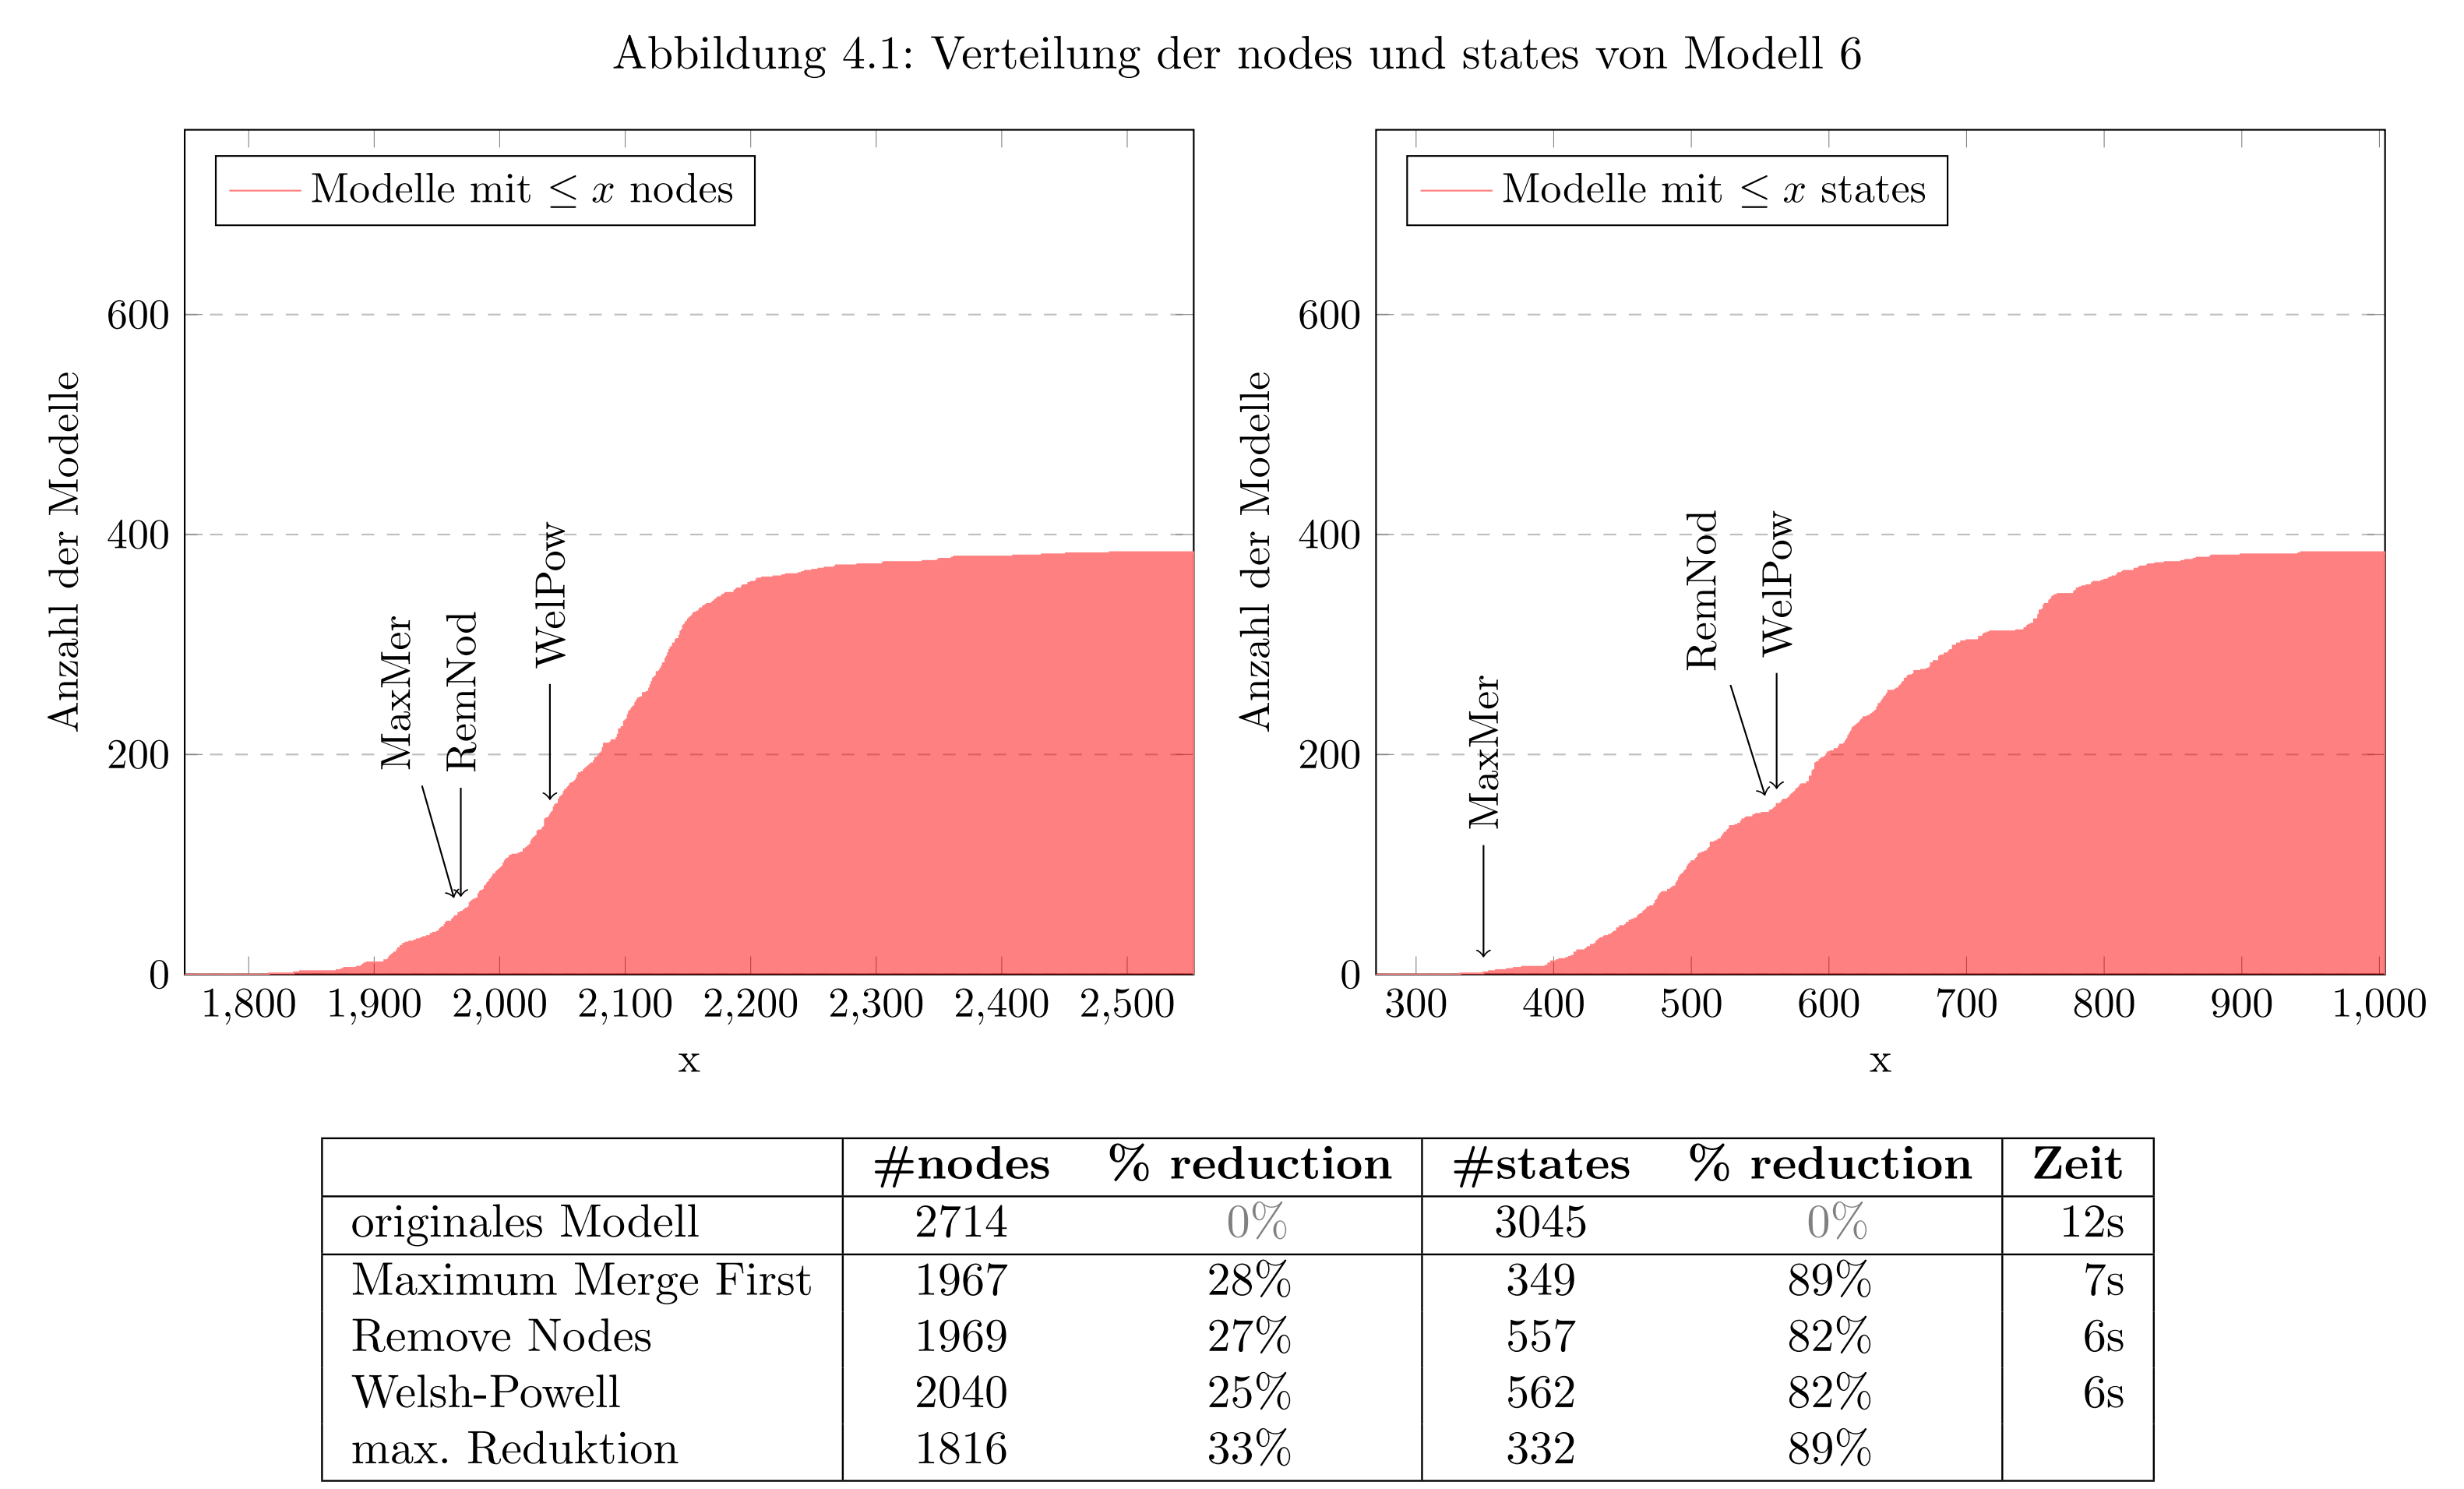
\includegraphics[scale=0.15]{m6.png}
}	
\end{frame}


\begin{frame}
	\frametitle{Ergebnisse Modell 11}
	\centering
	\makebox[0pt]{
		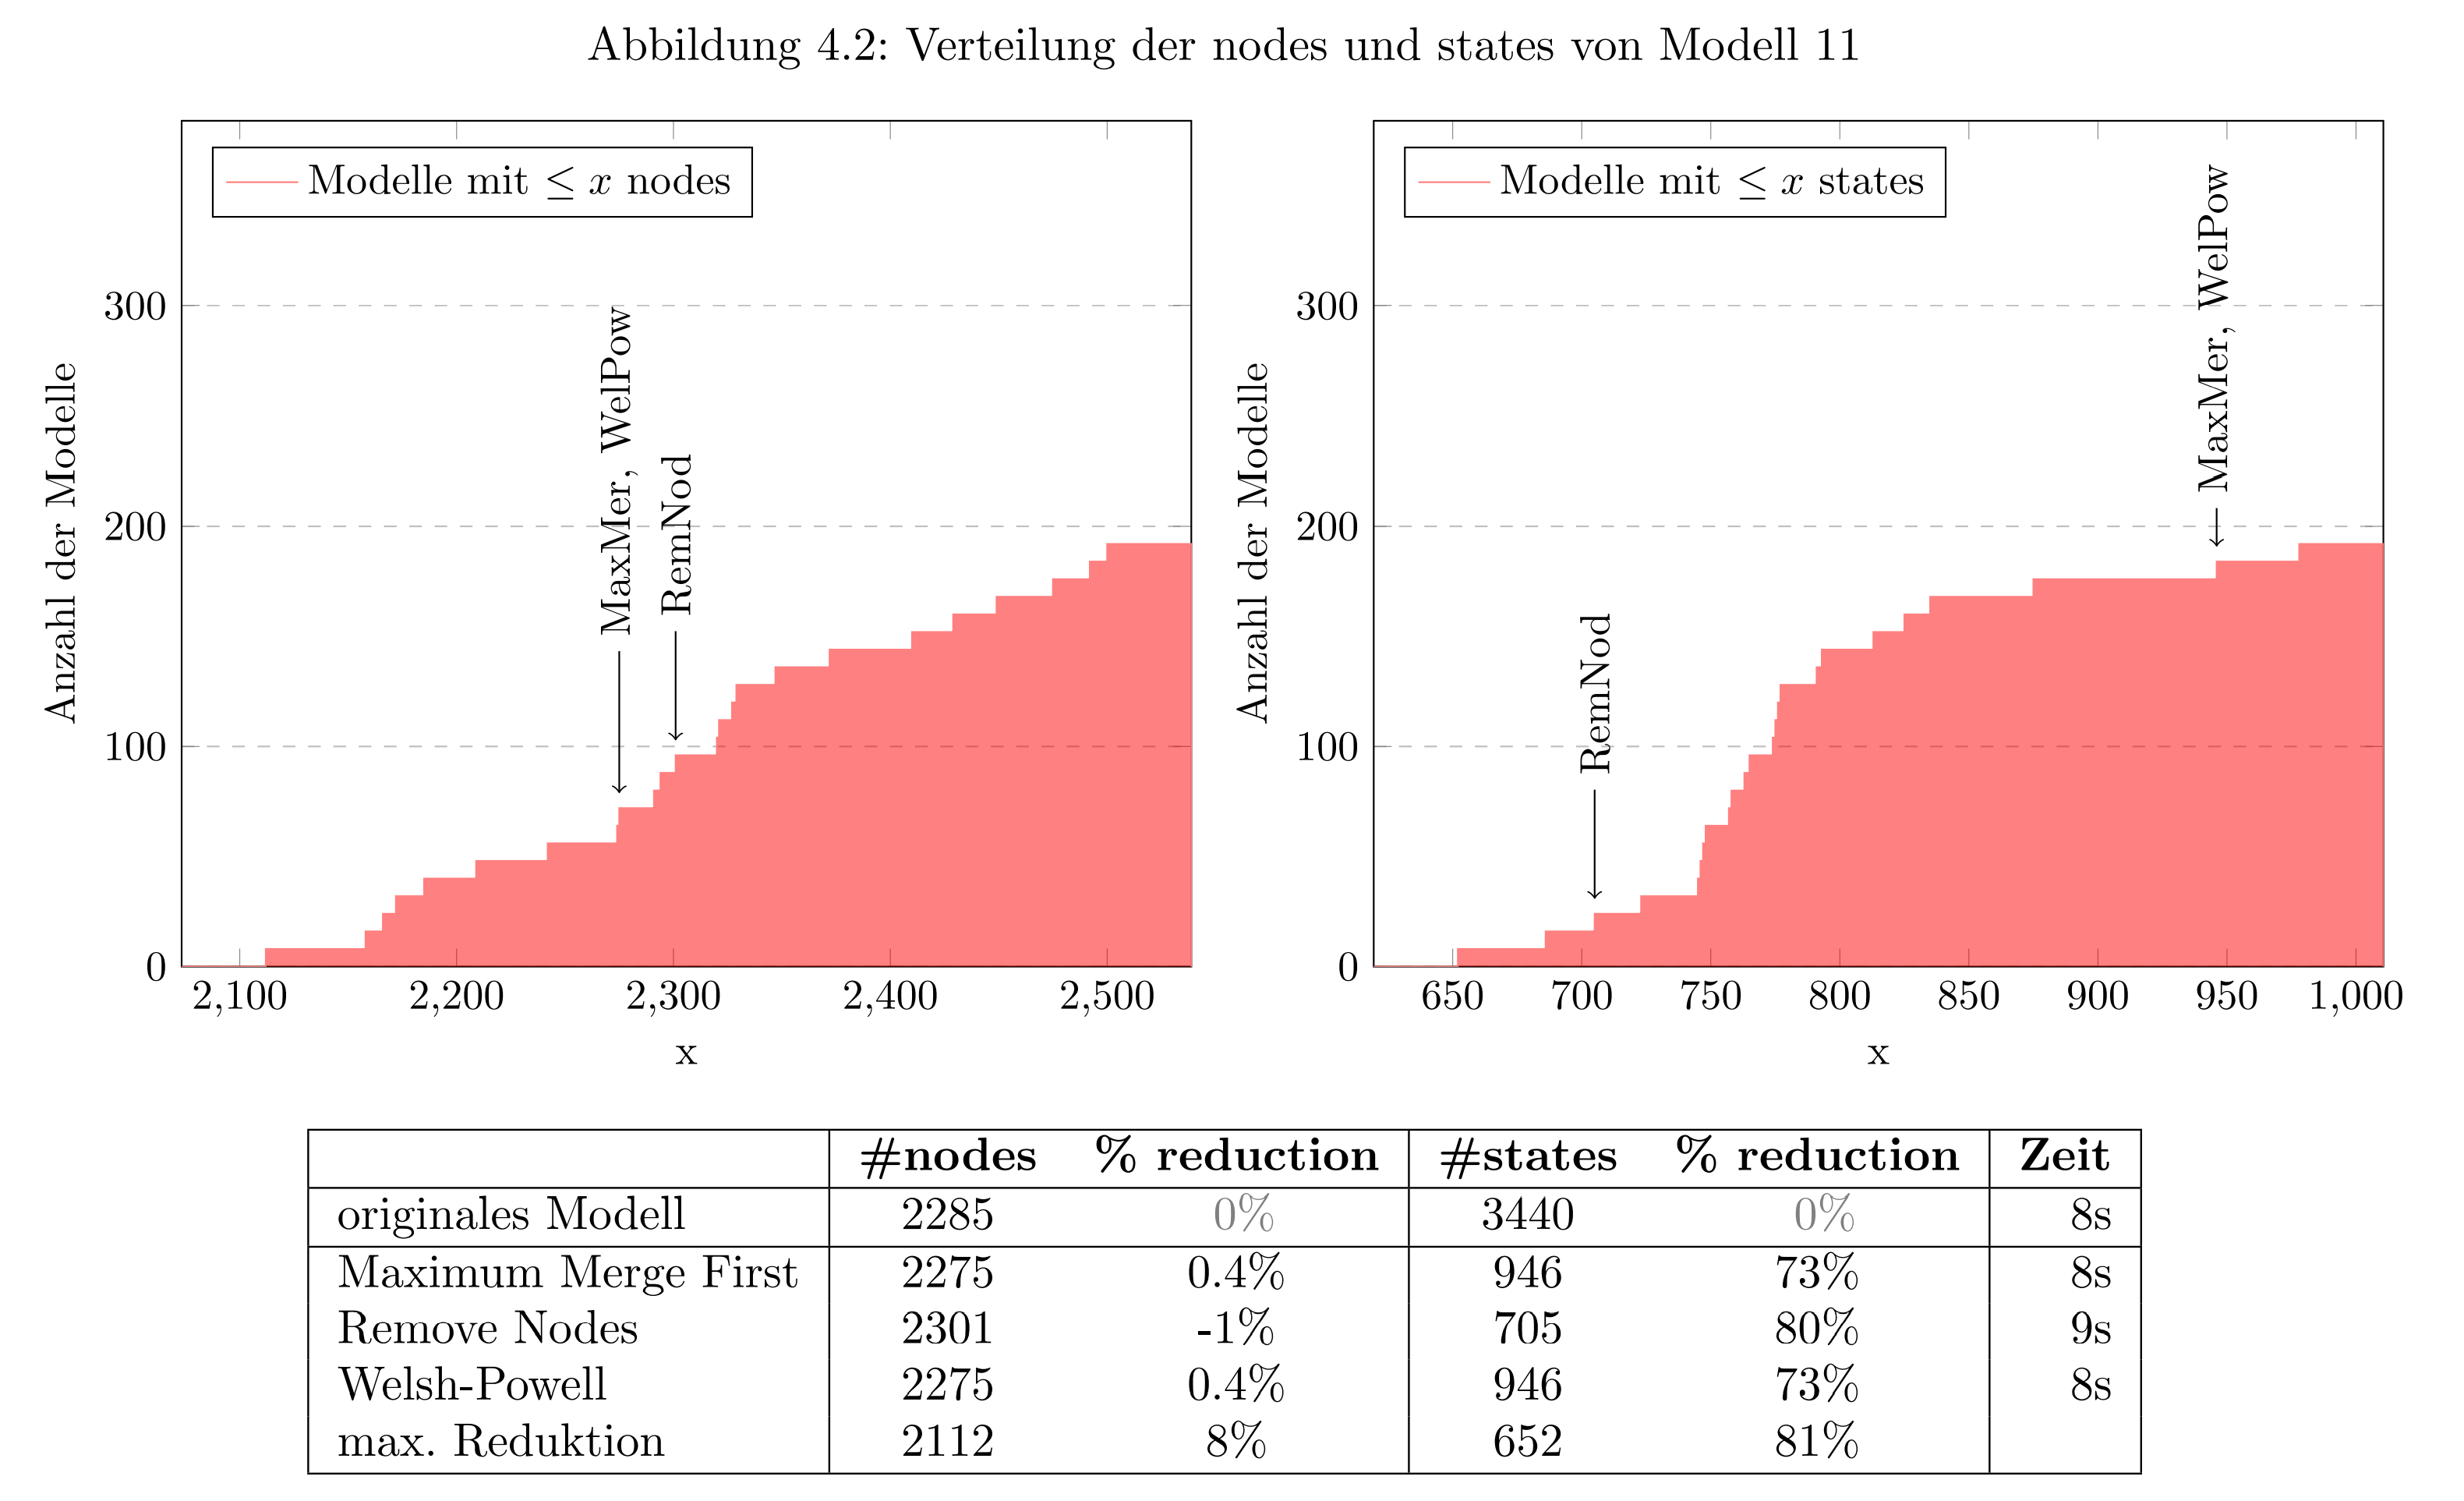
\includegraphics[scale=0.15]{m11.png}
	}	
\end{frame}

\begin{frame}
	\frametitle{Ergebnisse Modell 18}
	\centering
	\makebox[0pt]{
		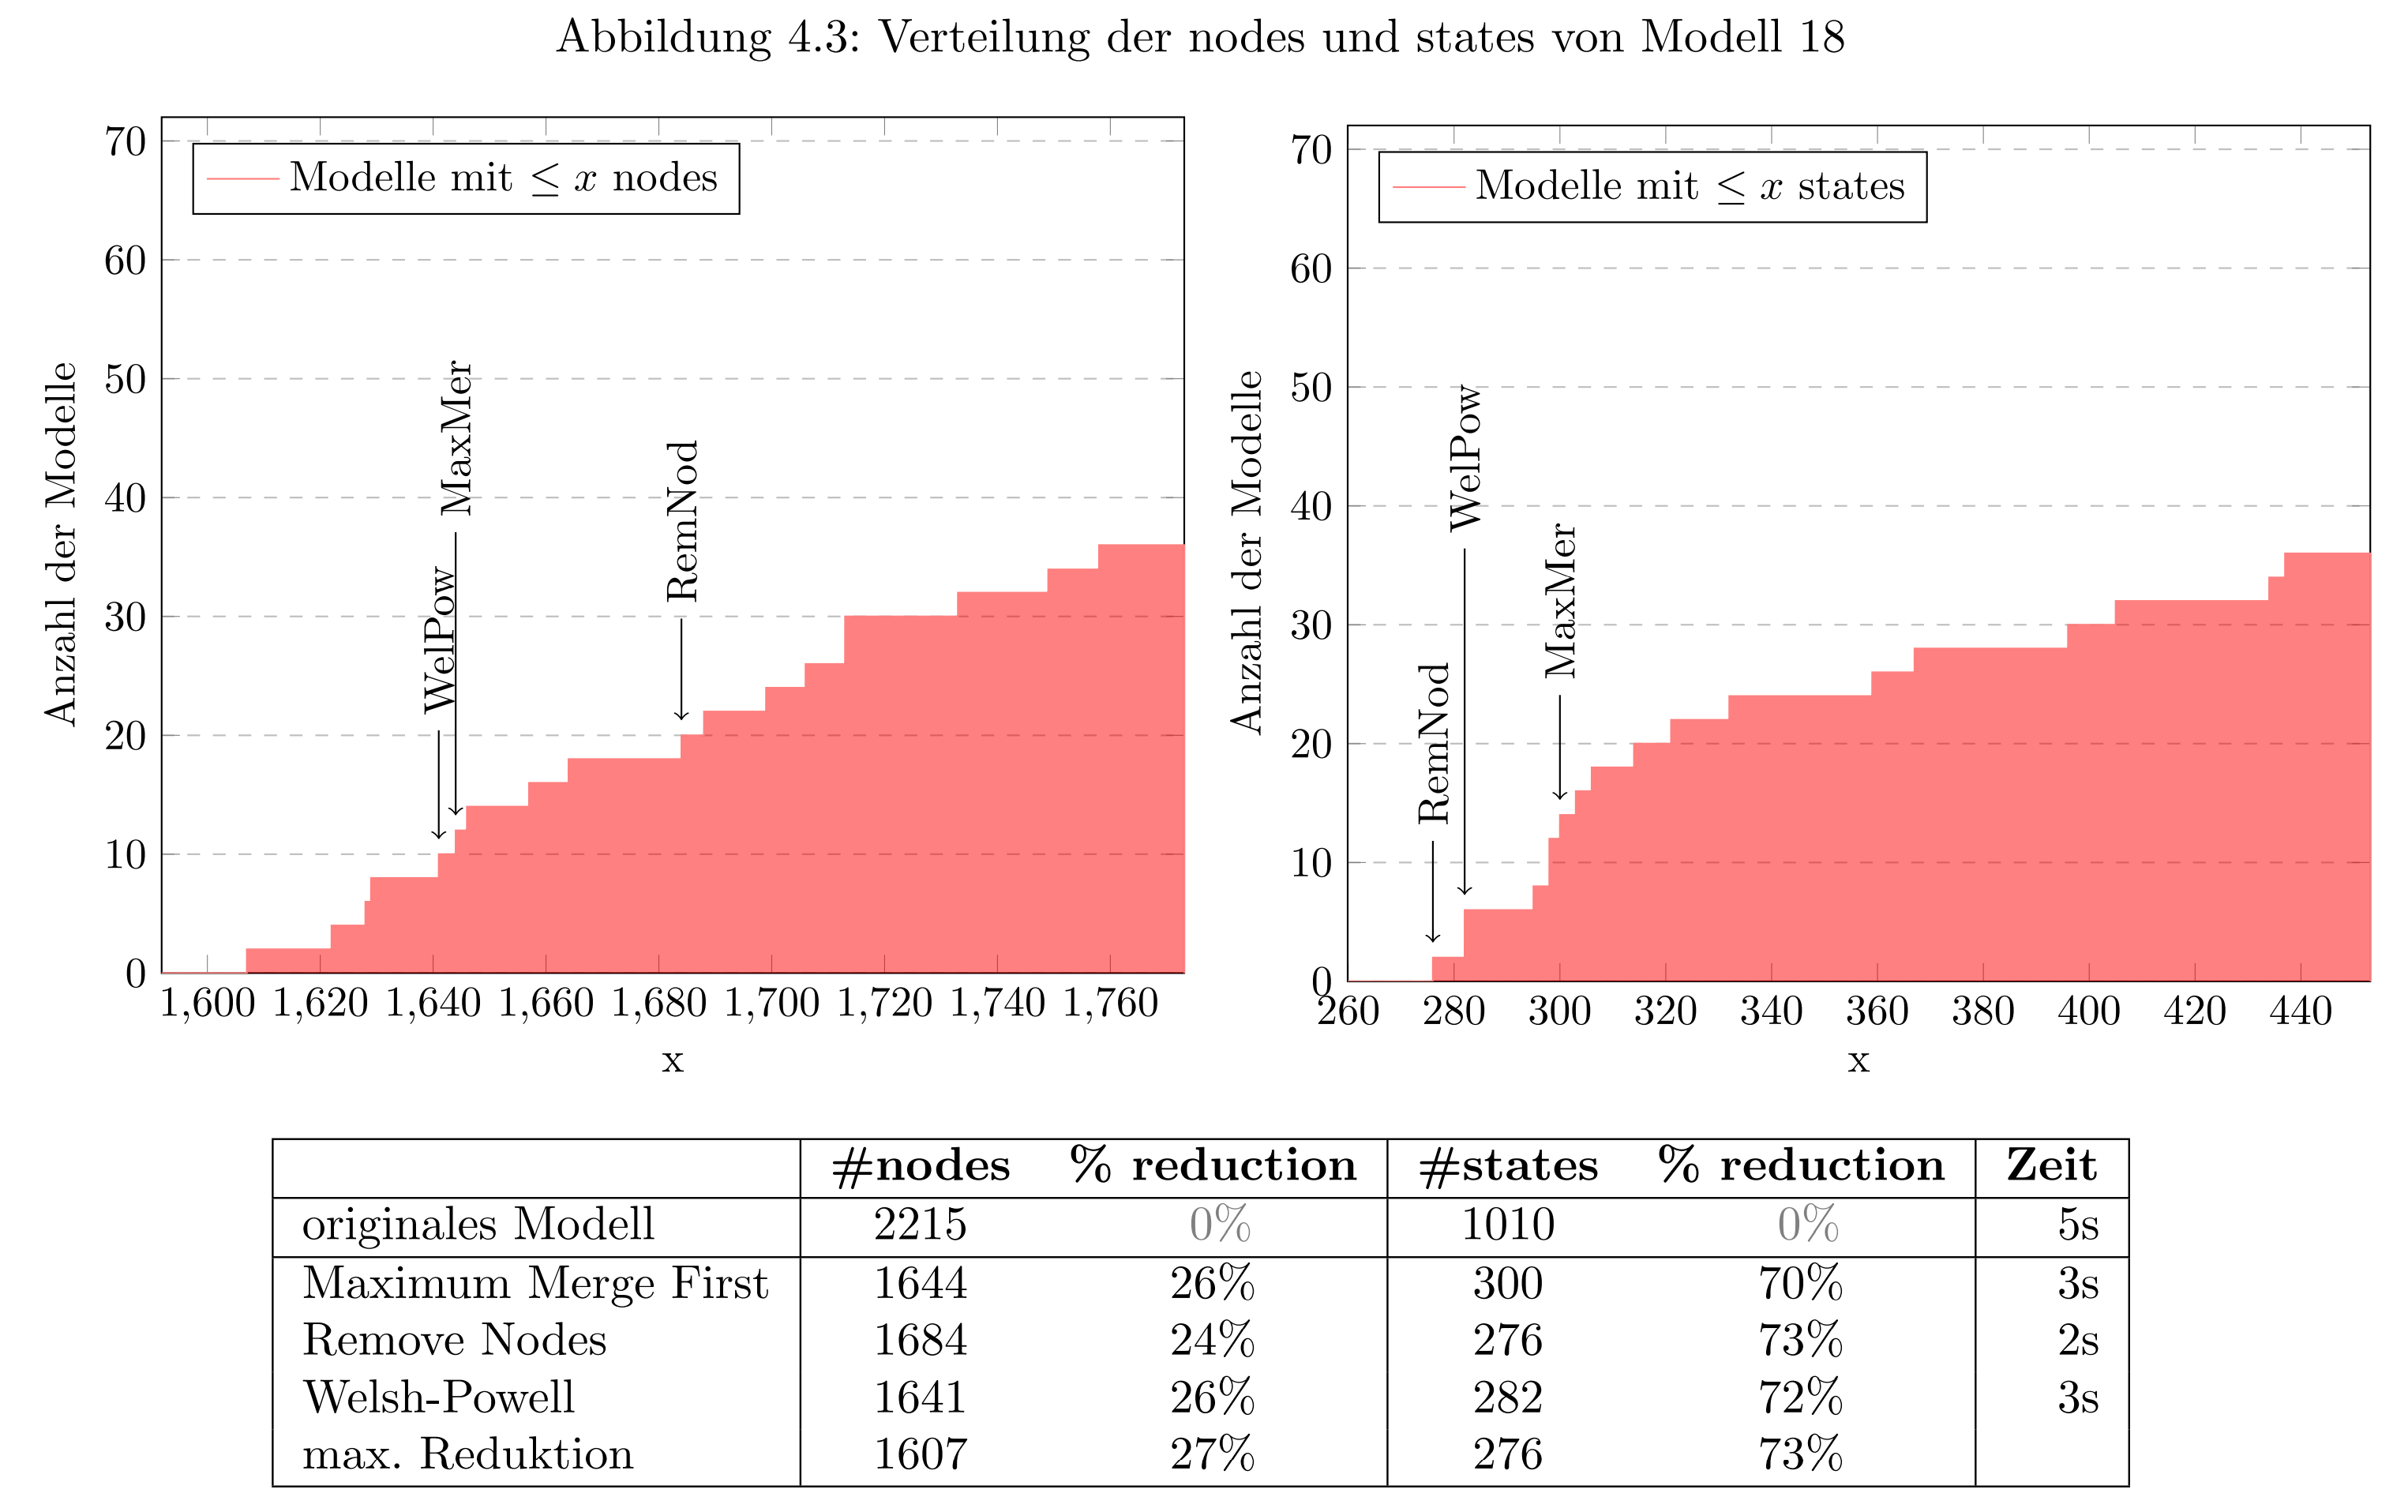
\includegraphics[scale=0.15]{m18.png}
	}	
\end{frame}

\begin{frame}
	\frametitle{Ergebnisse Modell in\_family}
	\centering
	\makebox[0pt]{
		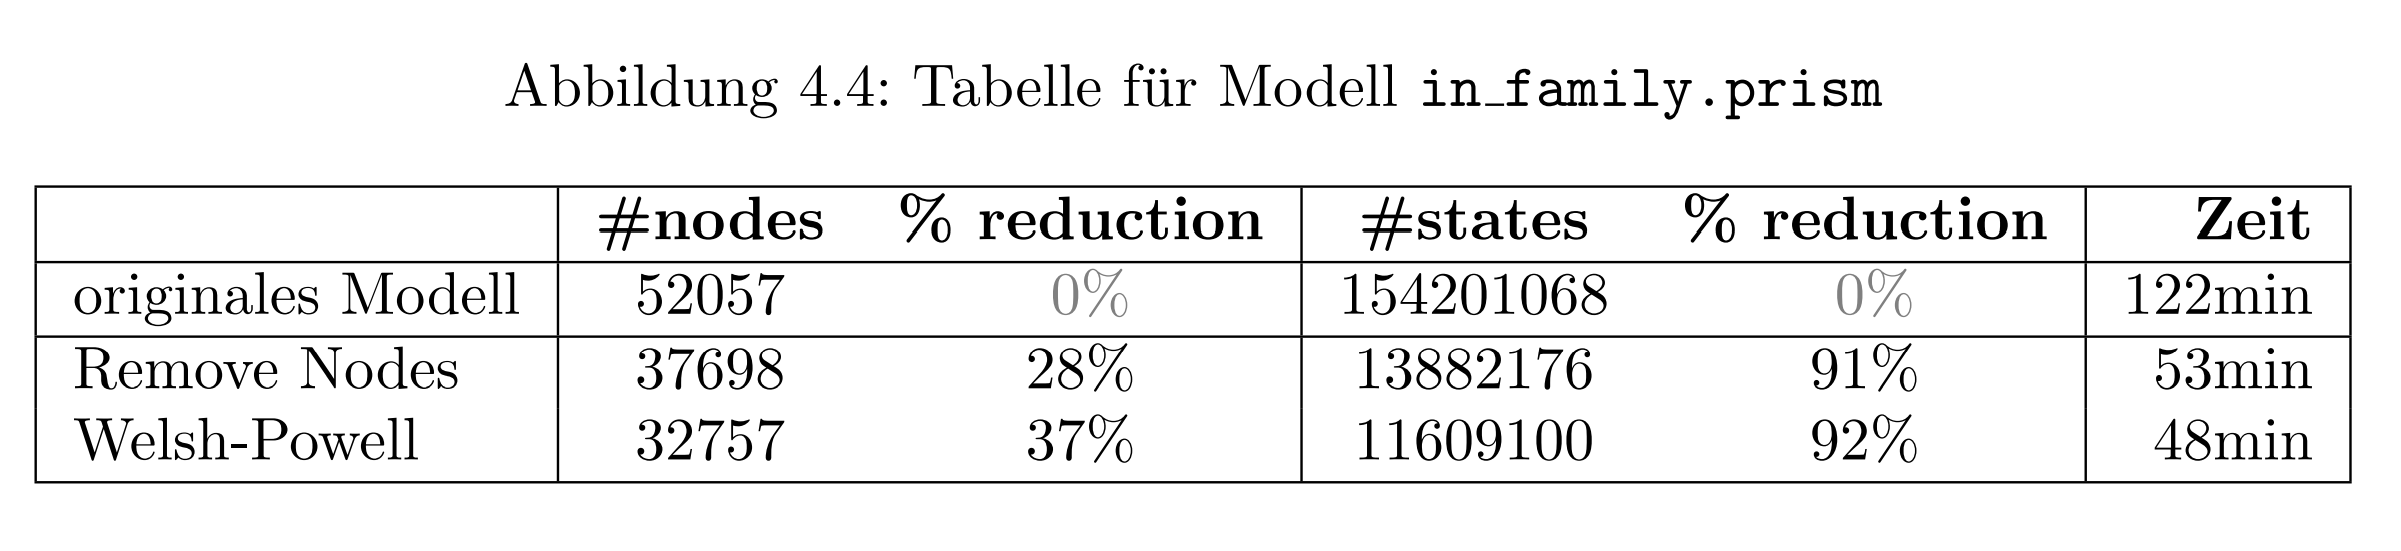
\includegraphics[scale=0.15]{fam.png}
	}	
\end{frame}

\section{Implementierung}

\begin{frame}
	\frametitle{grober Abriss}
	\begin{itemize}
		\item Parsen der Eingabesprache\pause
		\item Extrahieren des Multigraph\pause
		\item Live Range Analysis\pause
		\item Zwischenergebnis: ungerichteter Graph $H=(\mathrm{Var}, F)$\pause
		\item \textbf{Graphfärbung...}\pause \begin{itemize}
			\item Variablenkombinationen mit gleicher Färbung\pause
			\item Auswahl von Variablenkombinationen\pause
			\item Auflistung aller $k$-Färbungen, $k$ minimal
		\end{itemize}
	\end{itemize}	
\end{frame}

\begin{frame}
	\frametitle{Variablenkombinationen}
\begin{definition}[Variablenkombination]
	Wir nennen $k$ eine \emph{Variablenkombination}, wenn es ein Paar zweier boolscher Funktionen $k = (id, neighbours)$ ist mit
	\[id, neighbours : \mbox{Var} \to \{0,1\}
	\] \pause
	und $\neg \exists x \in \mathrm{Var} : id(x) = neighbours(x) = 1$. Wir nennen $size(k) \coloneqq |id|$ die \emph{Größe} der Variablenkombination. \pause
	Für ein Paar $k$ bezeichnen wir deren Elemente als $\mathrm{id}(k)$ und $\mathrm{neighbours}(k)$. Entsprechend gilt $k = (\mathrm{id}(k),\mathrm{neighbours}(k))$.
\end{definition} \pause

Jedem $x \in \mathrm{Var}$ ordnen wir die Variablenkombination $k_x \coloneqq (\{x\}, \{y \in \mathrm{Var} \mid \{x,y\} \in F\})$ zu.
\end{frame}

\begin{frame}
	\frametitle{Zusammenführbarkeit}

	\begin{definition}[zusammenführbar]
		Wir nennen zwei Variablenkombinationen $k, l$ \emph{zusammenführbar}, in Symbolen $k \downarrow l$, wenn \pause $\mathrm{id}(k) \cap \mathrm{neighbours}(l) = \emptyset$ und \pause $\mathrm{id}(l) \cap \mathrm{neighbours}(k) = \emptyset$. \pause Mit $k \cup l$ bezeichnen wir in diesem Fall die aus $k$ und $l$ nach Zusammenführen entstandene Variablenkombination  $k \cup l \coloneqq (\mathrm{id}(k) \cup \mathrm{id}(l), \mathrm{neighbours}(k) \cup \mathrm{neighbours}(l))$. \pause Aus Lesbarkeitsgründen verwenden wir hier die Schreibweise als Teilmengen von $\mathrm{Var}$.
	\end{definition}
\end{frame}

\begin{frame}
	\frametitle{Auflisten aller Variablenkombinationen}
	\begin{itemize}
		\item Sei $K_1 \coloneqq \{k_x \mid x\in \mbox{Var} \}$ \pause
		\item Dann berechnen wir $K_{i+1}$ aus $K_i$ und $K_1$ wie folgt: \pause
	\end{itemize} 
\centering
	\makebox[0pt]{
		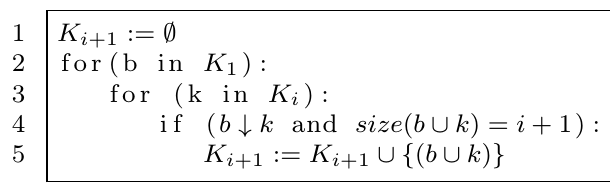
\includegraphics[scale=0.5]{vk.png}
	}	
\end{frame}

\begin{frame}
	\frametitle{Maximale Variablenkombinationen}
	\begin{itemize}
		\item Wir kennen $K_1, K_2, K_3, \dots $ \pause
		\item Dann berechnen wir $L_1, L_2, L_3 \dots$: \pause
	\end{itemize}
\begin{definition}[maximale Variablenkombination]
	Wir nennen eine Variablenkombination $k$ maximal, wenn es keine Variablenkombination $l\in K_1$ gibt, sodass $k, l$ zusammenführbar sind und $k \cup l \neq k$.
\end{definition} \pause
\begin{itemize}
	\item $L \coloneqq L_1 \cup L_2 \cup \dots \cup L_{max\_size}$
\end{itemize}
\end{frame}

\begin{frame}
	\frametitle{Abdeckung aller Variablen}
	\begin{itemize}
		\item Finde eine Auswahl $C \subseteq L$ mit $|C| = k$ mit \pause
		\begin{itemize}
			\item für jede Variable $x$ gibt es $(id, neighbours) \in C$, welches $x$ enthält, d.h. $id(x) = 1$.
		\end{itemize}
	\item Wir brauchen eine geschickte Implementierung!
	\end{itemize} \pause
\begin{definition}[Teilauswahl über $L$]
	Sei $L$ % = (l_1, l_2, \dots, l_n)$
	eine endliche Menge von Variablenkombinationen. Wir bezeichnen eine Abbildung
	\begin{equation*}
	c : L \to \{0, \#, 1\}
	\end{equation*}
	als \emph{Teilauswahl über} $L$. \pause Dabei nennen wir $l \in L$ \textit{ausgewählt} für den Fall $c(l) = 1$, \textit{nicht ausgewählt} für den Fall $c(l) = 0$ und \textit{nicht entschieden} für den Fall $c(l) = \#$.
\end{definition}
\end{frame}

\begin{frame}
	\frametitle{Auflistung aller minimalen Auswahlen}
	\centering
	\makebox[0pt]{
		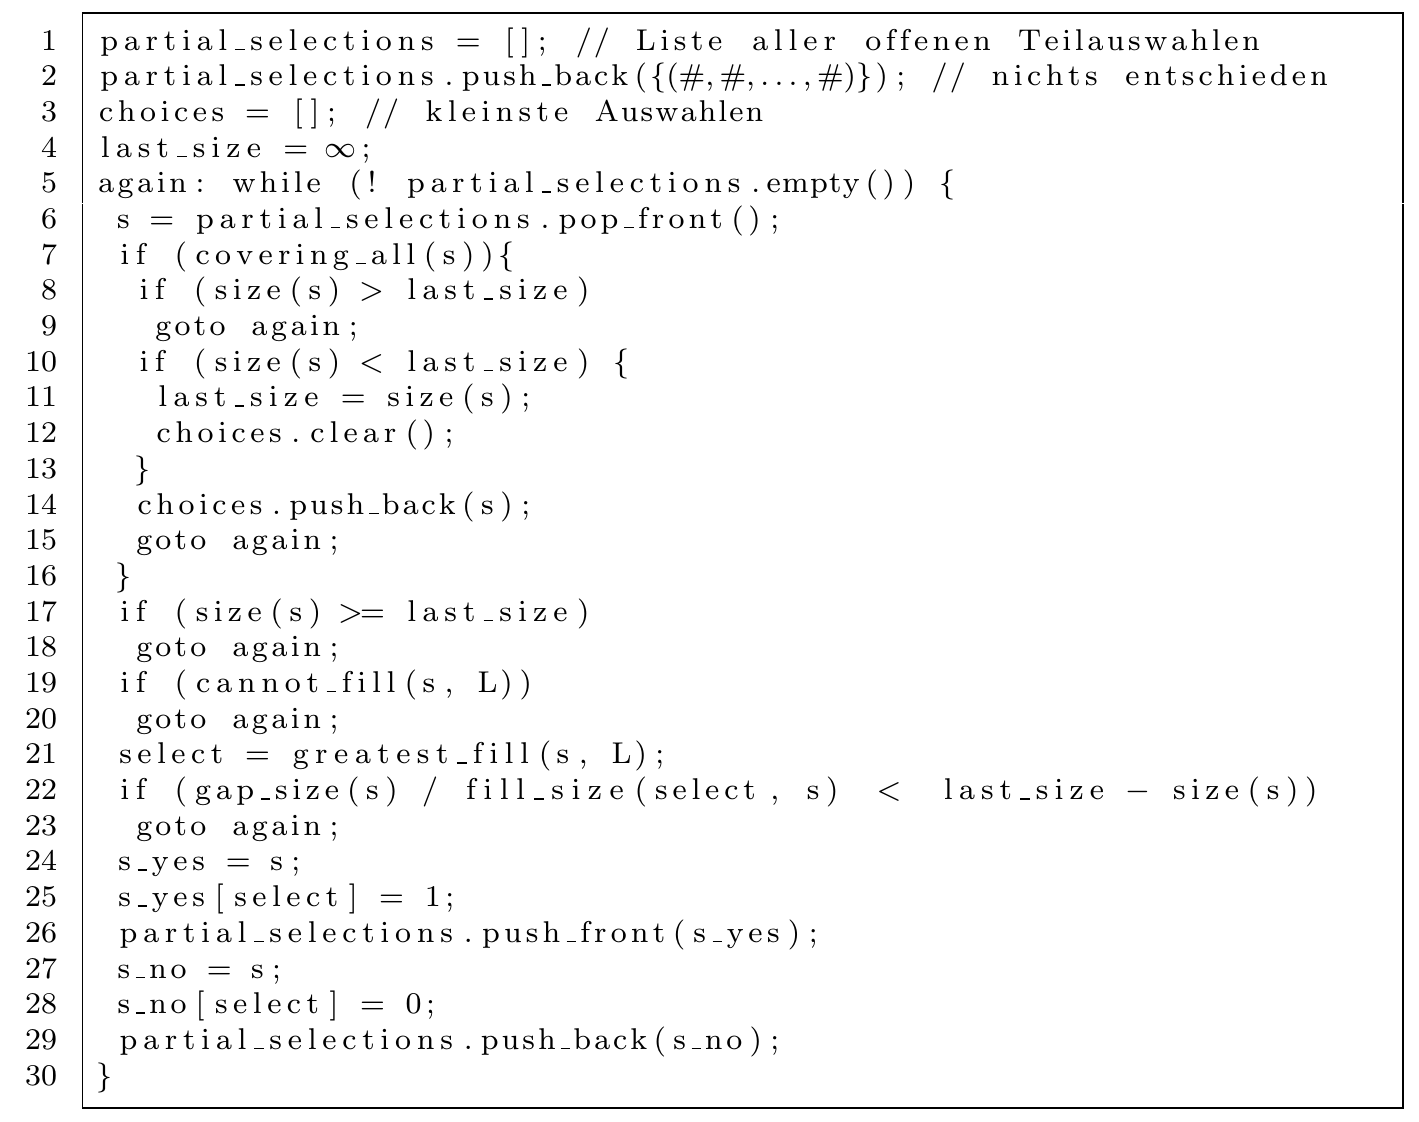
\includegraphics[scale=0.25]{choice.png}
	}	
\end{frame}


\begin{frame}
	\frametitle{Auflistung aller Graphfärbungen}
	\begin{itemize}
		\item mehrfach abgedeckte Variablen auflösen\pause
		\begin{itemize}
			\item Sehr viele Modelle können entstehen.
		\end{itemize} \pause
		\item Trick an vielen Stellen: Verwendung sortierter Arrays (\texttt{std::vector}) \pause
		
	\end{itemize}
\end{frame}

\begin{frame}
	\frametitle{Offene Fragen}
	\begin{itemize}
		\item Wie verteilen sich alle möglichen Resultate einer Heuristik?\pause
		\item Wann führen Heuristiken zu mehr Variablen als nötig?
	\end{itemize}
\end{frame}

\end{document}